\subsection{XoR}
\label{exo:XoR}

keywords: strength augmentation; hybrid actuation\\

\begin{figure}[ht]
  \centering
  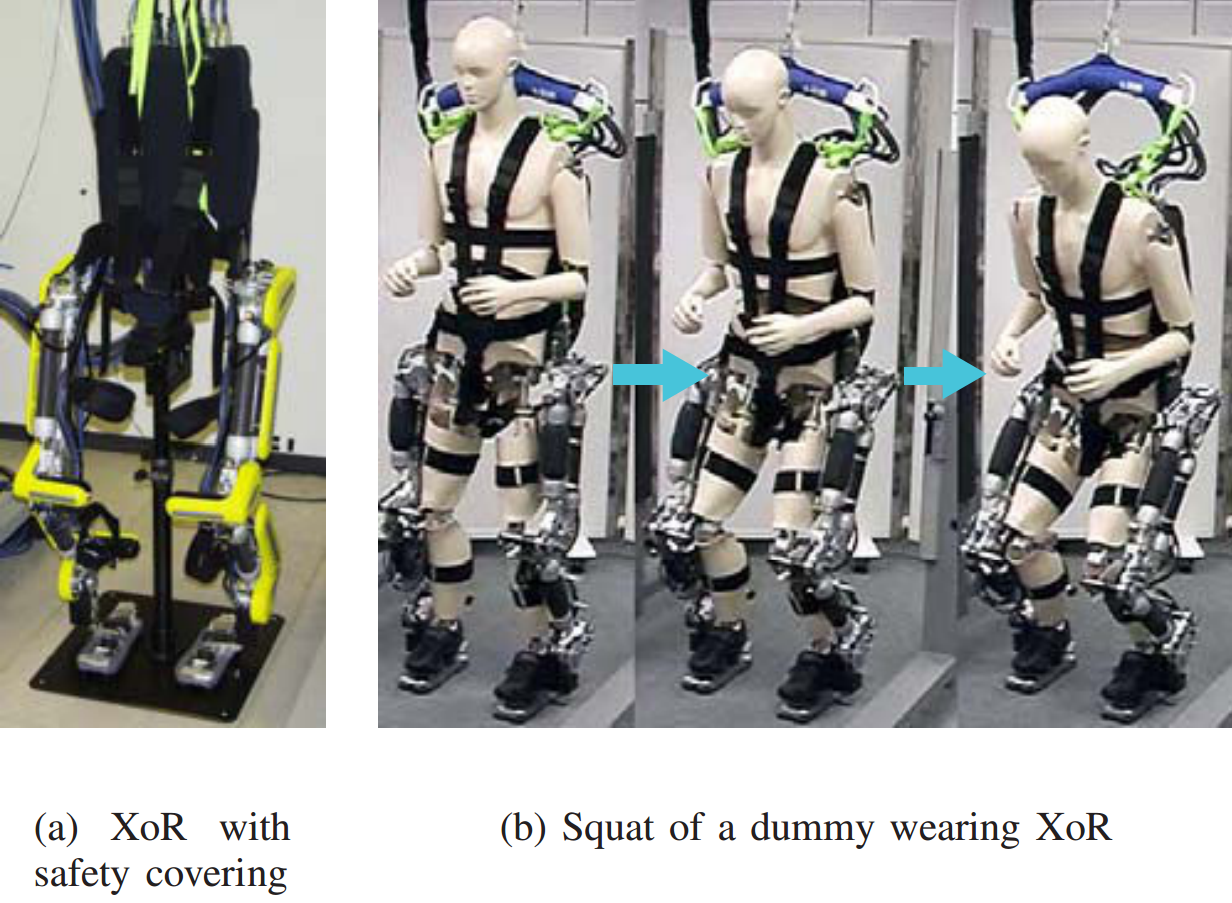
\includegraphics[width=4.0in]{exos/figs/xor.png}
\end{figure}


muscular weakness

Purpose: prototype developed for "postural control of elderly people and persons with mobility disability" -- [[llimbCtrlReviw]]


Design:

"implements a hybrid driving concept combining pneumatic artificial muscles and electric motors together [[XoRdesign]]; [[XoRkinemExtraction]] ...motion intention is estimated based on EMG signals ... user posture based on joint angles and ground reaction forces."  -- [[llimbCtrlReviw]]


Control Strategy:

Model-based control -- "...Pneumatic artificial muscles provide gravity compensation and electric motors serve the dynamic compensator. The total generated torque tracks a desired value calculated on the basis of a bio-mechanical model... Only simulation results were available to prove the efficacy of this assistive strategy working with XoR." -- [[llimbCtrlReviw]]


References:

S. Hyon, J. Morimoto, T. Matsubara, T. Noda, M. Kawato, Xor: Hybrid drive exoskeleton robot that can balance, in: Intelligent Robots and Systems (IROS), 2011 IEEE/RSJ International Conference on, IEEE, 2011, pp. 3975–3981. <<XoRdesign>>

J. Morimoto, T. Noda, S. Hyon, Extraction of latent kinematic relationships between human users and assistive robots, in: Robotics and Automation (ICRA), 2012 IEEE International Conference on, IEEE, 2012, pp. 3909–3915. <<XoRkinemExtraction>>


***** Data from design paper [[XoRdesign]]

HMI: 
Brain-machine interface.

Acutation:  
Hybrid drive - pneumatic muscles with electrical motors arranged in "optimal ways."

Design criteria:

Precise torque control; high backdrivability; force/velocity profile for rehab and compensation; lightweight; quasi-autonomy for rehab; autonomous posture control.

Precise torque control -- they believe this is most important feature to mobility assist/rehab programs as softness, compliance, and safety are defined in force/toque space;

safety thru passive backdrivability;

air muscles -- use them because there is negligable stick-slip; better controllability but gnereated force decreases quadratically with contraction (vanish around 30% contraction); optimize arrangment of AM to generate desired forces in specific confgs.  Use air muscle (AM) as gravity compensator and electric motor as dynamic compensator.  AM has high power density; good for high-load torque but delayed due to air compressibility.  There is also steady-state error.  Electric motors (without gear reduction) have high response torque but can only generate for short periods.  Hybrid drive sums the two to produce desired torque profile.  Can combine AM with small electric servos or hydraulic servo actuators.  Small servos without high gear reduction; DC (brushed and brushless).  

Use AM as a unilateral drive for gravity comp combined with bilateral electric motors (motion control); generates precise high torque.  The air compressor / hydraulic pump can be smaller and lighter electric batteries.

10 DOF; 6 active (all FE joints with hybrid drive) and 6 passive joints (hip ankle AA, hip rotation);

Transmission - AM connected to pulleys via tendons.  Rubber muscle (MDSP-40) with EP regulators mounted in backpack; testing constant pressure and cam to reduce weight required for backpack air valves.  Bruschless DC geared motors (4.7 A rating; 0.12Nm output; gear ratio 57.5 for backdrivability; for short operation motor can generate 34.5 Nm/joint) with belt and pulleys

Range of motion of 120 deg and load capacity 150 Nm.  Weight 33kg of which toro + cables ~15kg. Experiments show insufficient torque and need for bi-directional pneumatic acuation at hip joints.

Sensing -- Rotory encoders at each joint; IMU in backpack; load cells at feet; network connected with servers processing sensory info from EMG, NIRS and EEG.  Controller runs at 1ms on Linux PC.


Control:

PLANNED: Torque control; apply compliant control mechanisms designed for full humanoid to exoskeleton control

S. Hyon, “Compliant terrain adaptation for biped humanoids without
measuring ground surface and contact forces,” IEEE Trans. Robotics,
vol. 25, no. 1, pp. 171–178, 2009.

S. Hyon, “A motor control strategy with virtual musculoskeletal
systems for compliant anthropomorphic robots,” IEEE/ASME Transactions
on Mechatronics, vol. 14, issue 6, pp. 677–688, 2009.

In simulation:
Task-space controller; The paper describes CoM / CoP control strategy based on GRF.  Achieve desired GRF using PD feedback to track desired COM trajectory.  Full-body task space controller superimposed with a joint stiffness controller applying feedback tracking ref joint trajectories.  Simulations reveal max torque of 150 Nm (effective torque of 80Nm) for HFE and KFE joints.  Plan to include EMG sensors;

------------------------------------------------

\subsection{Assessment and Recommendations}

The XoR prototype uses a novel hybrid actuation scheme to achieve both fast peak torque response and high sustained torque.  


% \bibliographystyle{plain}
% \bibliography{exos/xor}

The figures in this section were obtained from \cite{xorDesign2011}. Materials presented are based on the references above.